\section{Cálculo de parámetros $\frac{W}{L}$ del amplificador tipo \textit{folded cascode} \label{sec:s3}}

\begin{center}
	\begin{minipage}{12cm}
		\begin{tcolorbox}[title=Actividad 2]
			Emplear la siguiente metodología, propuesta por \cite{Allen_2012} para diseñar el amplificador \textit{folded cascode} de una etapa (Ver \autoref{fig:calculos_folded}).
		\end{tcolorbox}	
	\end{minipage}
\end{center}

\begin{figure}[H]
	\centering
	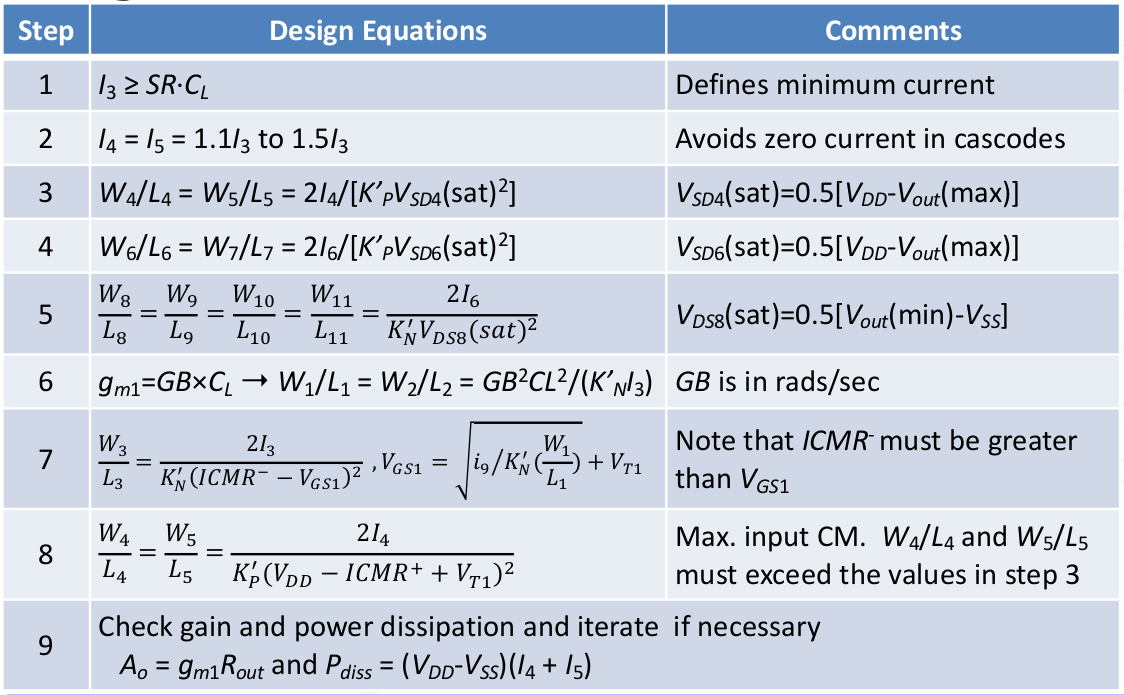
\includegraphics[scale=0.34]{Calculos_Folded.png}
	\caption{Procedimiento de diseño del amplificador \textit{folded cascode}. \label{fig:calculos_folded}}
\end{figure}

\begin{equation*}
	\begin{array}{l l}
		\textbf{Parametros conocidos} \\
		V_{DD} =  1.8  V \\
		V_{SS} =  0  V \\
		L_{min} =  450.0  nm \\
		0.8 V \leq ICMR \leq 1.8 V \\
		K'_{N} =  151.37604  \frac{\mu A}{V^{2}} \\
		K'_{P} =  57.013889  \frac{\mu A}{V^{2}} \\
		V_{TN} =  0.769432  V \\
		V_{TP} =  0.624345  V \\
		\lambda_{N} =  0.088964  V^{-1} \\
		\lambda_{P} =  0.068964  V^{-1} \\
		C_{L} =  15.0  pF \\
		\\
		\textbf{Características deseadas} \\
		A_{V} =  3000  \frac{V}{V} \\
		P_{diss} \leq  1.0  mW \\
		GB =  10.0  MHz \\
		SR \geq  5  \frac{V}{\mu s} \\
		0.3 V \leq V_{OUT} \leq 1.4 V \\
		\\
		\textbf{Paso 1} \\
		I_{3} = SR \times C_{L} = 10\times1.5e-11 \\
		I_{3} =  150.0 \mu A \\
		I_{1} = \frac{I_{3}}{2} = \frac{ 0.00015 }{2} \\
		I_{1} = I_{2} =  75.0 \mu A \\
		\\
		\textbf{Paso 2} \\
		I_{4} = 1.1 \times I_{3} = 1.1 \times 150.0  \\
		I_{4} = I_{5} =  165.0 \mu A \\
		\\
		\textbf{Paso 3} \\
		V_{SD4}(sat) = 0.5 \times \left[ V_{DD} - V_{OUT}(max) \right] = 0.5 \times \left[  1.8  -  1.4  \right] \\
		V_{SD4} = V_{SD5} =  0.2  V \\
		\frac{W_4}{L_4} = \frac{2\times I_{4}}{K'_{P}\times V_{SD4}(sat)^2} = \frac{2\times 0.000165 }{ 5.7e-05 \times ( 0.2 )^2} \\
		\frac{W_4}{L_4} =  144.701583  \\
		W_{4} = \frac{W_4}{L_4} \times L_{min} =  144.701583 \times 4.5e-07  \\
		W_{4} = W_{5} =  65.115712  \mu m \\
	\end{array}
\end{equation*}

\begin{equation*}
	\begin{array}{l l}
		\textbf{Paso 4} \\
		\text{Se asume que } I_{7} = I_{6} = I_{4} =  165.0 \mu A \\
		\text{Por lo tanto } \frac{W_7}{L_7} = \frac{W_6}{L_6} = \frac{W_4}{L_4} =  144.701583  \\
		W_{7} = W_{6} = W_{5} = W_{4}=  65.115712  \mu m \\
		\\
		\textbf{Paso 5} \\
		\text{Se asume que } I_{8} = I_{4} =  165.0 \mu A \\
		V_{DS8}(sat) = 0.5 \times \left[ V_{OUT}(min) - V_{SS} \right] = 0.5 \times \left[  0.3  -  0  \right] \\
		V_{DS8}(sat) =  0.15  V \\
		\frac{W_8}{L_8} = \frac{2\times I_{8}}{K'_{N}\times V_{DS8}(sat)^2} = \frac{2\times 0.000165 }{ 0.000151 \times ( 0.15 )^2} \\
		\frac{W_8}{L_8} =  96.888957  \\
		W_{8} = \frac{W_8}{L_8} \times L_{min} =  96.888957 \times 4.5e-07  \\
		W_{8} = W_{9} = W_{10} = W_{11} =  43.600031  \mu m \\
		\\
		\textbf{Paso 6} \\
		\frac{W_1}{L_1} = \frac{\left( GB^2 \times C_{L}^2 \right)}{K'_{N} \times I_{3}} = \frac{\left(  10000000.0 ^2 \times  1.5e-11 ^2 \right)}{ 0.000151  \times  0.00015 } \\
		\frac{W_1}{L_1} =  0.99091  \\
		W_{1} = \frac{W_1}{L_1} \times L_{min} =  0.99091 \times 4.5e-07  \\
		W_{1} = W_{2} =  0.445909  \mu m \\
		\\
		\textbf{Paso 7} \\
		V_{DS3}(sat) = \sqrt{\frac{I_{3}}{K'_{N} \times \frac{W_1}{L_1}}} - V_{TN} = \sqrt{\frac{ 0.00015 }{ 0.000151  \times  0.99091 }} -  0.769432  \\
		V_{DS3}(sat) =  0.230568  V \\
		\frac{W_3}{L_3} = \frac{2\times I_{3}}{K'_{N} \times V_{DS3}(sat)^2} = \frac{2\times 0.00015 }{ 0.000151 \times ( 0.230568 )^2} \\
		\frac{W_3}{L_3} =  37.279154  \\
		W_{3} = \frac{W_3}{L_3} \times L_{min} =  37.279154 \times 4.5e-07  \\
		W_{3}  =  16.775619  \mu m \\
		\\
		\textbf{Paso 8} \\
		\frac{W_4}{L_4}_{spec} = \frac{2\times I_{4}}{K'_{P} \times \left( V_{DD} - ICMR^{+} + V_{TN} \right) ^2} = \frac{2 \times  0.000165 }{ 5.7e-05  \times \left(  1.8  -  1.8  +  0.769432  \right) ^2} \\
		\frac{W_4}{L_4}_{spec} =  9.776711  \\
		\text{Se observa que } \frac{W_4}{L_4} \geq \frac{W_4}{L_4}_{spec} \text{ por lo que la relación } \frac{W_4}{L_4} \text{ esta bien calculada.} \\
	\end{array}
\end{equation*}

\begin{equation*}
	\begin{array}{l l}
		\textbf{Paso 9} \\
		I_{T} = I_{4} + I_{5} =  0.000165 + 0.000165  \\
		I_{T} =  330.0  \mu A \\
		P_{diss} = (V_{DD} - V_{SS}) \times I_{T} = ( 1.8 - 0 ) \times  0.00033  \\
		P_{diss} =  0.594  mW \\
		g_{m1} = \sqrt{2 \times I_{1} \times K'_{N} \times \frac{W_1}{L_1}} = \sqrt{2 \times  7.5e-05  \times  0.000151  \times  0.99091 } \\
		g_{m1} =  150.0  \mu S \\
		g_{m4} = \sqrt{2 \times I_{4} \times K'_{P} \times \frac{W_4}{L_4}} = \sqrt{2 \times  0.000165  \times  5.7e-05  \times  144.701583 } \\
		g_{m4} =  1650.0  \mu S \\
		g_{m6} = \sqrt{2 \times \left( \frac{I_{T} - I_{3}}{2} \right) \times K'_{P} \times \frac{W_4}{L_4}} = \sqrt{2 \times \left( \frac{ 0.00033  -  0.00015 }{2} \right) \times  5.7e-05  \times  144.701583 } \\
		g_{m6} =  1218.605761  \mu S \\
		g_{m8} = \sqrt{2 \times \left( \frac{I_{T} - I_{3}}{2} \right) \times K'_{N} \times \frac{W_8}{L_8}} = \sqrt{2 \times \left( \frac{ 0.00033  -  0.00015 }{2} \right) \times  0.000151  \times  96.888957 } \\
		g_{m8} =  1624.807681  \mu S \\
		r_{ds1} = \frac{1}{\lambda_{N} \times I_{1}} = \frac{1}{ 0.088964  \times  7.5e-05 } \\
		r_{ds1} =  149.873807  K \Omega \\
		r_{ds4} = \frac{1}{\lambda_{P} \times I_{4}} = \frac{1}{ 0.068964  \times  0.000165 } \\
		r_{ds4} =  87.881062  K \Omega \\
		r_{ds6} = \frac{1}{\lambda_{P} \times \left( \frac{I_{T} - I_{3}}{2} \right)} = \frac{1}{ 0.068964  \times \left( \frac{ 0.00033  -  0.00015 }{2} \right)} \\
		r_{ds6} =  161.11528  K \Omega \\
		r_{ds8} = \frac{1}{\lambda_{N} \times \left( \frac{I_{T} - I_{3}}{2} \right)} = \frac{1}{ 0.088964  \times \left( \frac{ 0.00033  -  0.00015 }{2} \right)} \\
		r_{ds8} =  124.894839  K \Omega \\
		R_{OUT} = \left( g_{m8} \times r_{ds8}^{2} \right) || \left[ g_{m6} \times r_{ds6} \times \left( r_{ds1} || r_{ds4} \right) \right] \\
		R_{OUT} = \left(  0.002  \times  124894.839 ^{2} \right) || \left[  0.001  \times  161115.28  \times \left(  149873.807  ||  87881.062  \right) \right] \\
		R_{OUT} =  13.616628  M \Omega \\
		A_{0} = g_{m1} \times R_{OUT} =  0.00015  \times  13616627.980708  \\
		A_{0} =  2042.494197  =  66.203217  db \\
		\\
		\textbf{Parámetros calculados} \\
		W_{1} = W_{2} =  0.446  \mu m \\
		W_{3} =  16.776  \mu m \\
		W_{4} = W_{5} = W_{6} = W_{7} =  65.116  \mu m \\
		W_{8} = W_{9} = W_{10} = W_{11} =  43.6  \mu m \\
		L_{1} - L_{11} =  0.45  \mu m \\
	\end{array}
\end{equation*}